%-----------------------------------------------------
\subsubsection{Perspectiva general de la investigación}
%-----------------------------------------------------

\begin{frame}
\frametitle{Perspectiva general}
%------------------------------
\begin{columns}

    \begin{column}{0.50\textwidth}
    \vspace{-5pt}
    \begin{block}{\textcolor{blue}{Oferta}}
        \begin{column}{0.1\textwidth}
        \vspace{-10pt} % estos espacios negativos son claves para alinear
            \tiny
            \begin{align*}
            c_{1,t}+\Phi_t \le y\\
            c_{2,t+1}\le\Phi_{t+1}^R\\
            N_{t-1}\textcolor{red}{x_t} \cdot \Phi_{t-1}^{\textbf{DLT}}=N_t(*)
            \end{align*}
        \end{column}
        \begin{column}{0.35\textwidth}  
            \begin{figure}[H]
            \begin{center}
             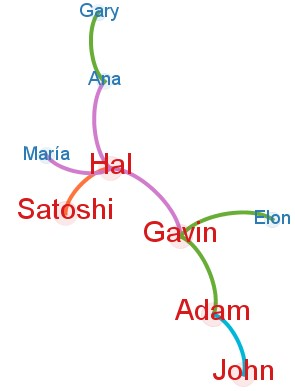
\includegraphics[width=1\textwidth]{images/C2/c2_simul_red5.jpg}
             \end{center}
            \end{figure}
            \end{column}
    \end{block}
    \begin{block}{\textcolor{dgreen}{Demanda}}
        \vspace{-10pt}
            \tiny
              \begin{align*}
              v_{t}^{\$}{M_{t}^{\$}}&={N_{t}^{\$}\left(*\right)}+(1-\lambda_t){N_{t}^{\$}\left(*\right)}\\
              v_{t}^{\bitcoinA}{M_{t}^{\bitcoinA}}&={N_{t}^{\bitcoinA}\left(*\right)+\lambda_tN_{t}^{\$}\left(*\right)}\\
              \lambda_t&=\textcolor{blue!70}{S}(\textcolor{red}{\mu_t})
            \end{align*}
    \vspace{-20pt}
            \begin{figure}[t!]
            \begin{center}
            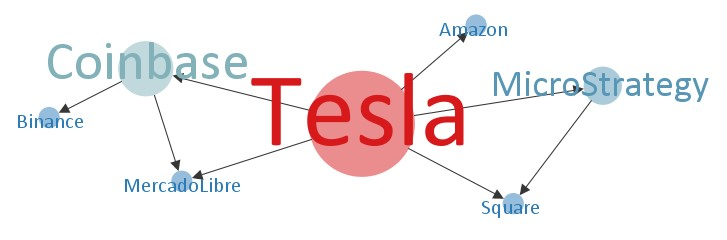
\includegraphics[width=0.6\textwidth]{images/C3/c3_simul_influ3.jpg}
             \end{center}
            \end{figure}
            
    \end{block}
    \end{column}
    
    \begin{column}{0.55\textwidth}
    
    \begin{block}{\textcolor{orange}{Implicancias}}
    \tiny

    \begin{align*}
    v^{\$a}_1 M^{\$a}_1&=P_1^{{\$a}} + \lambda_1 (1-\alpha_1) R_1^{{\$a}} + (1-\lambda_1) \textcolor{blue!60}{\rho_1}  R_1^{{\$a}}\\
    v_1^{\$} M_1^{\$}&=(1-\lambda_1) \textcolor{green!70}{\delta_1} R_1^{\$a}\\
    v_1^{\bitcoinA} M_1^{\bitcoinA}&=\textcolor{orange}{\lambda_1}  \alpha_1 R_1^{\$a} + (1-\lambda_1) \textcolor{red}{\beta_1} R_1^{\$a}\\
    e_t^{{\$a};{\$}}&=\frac{v_1^{\$a}}{v_1^{\$}}
    \end{align*}
    
    \vspace{-5pt}
    
    \begin{figure}[H]
    \begin{center}
     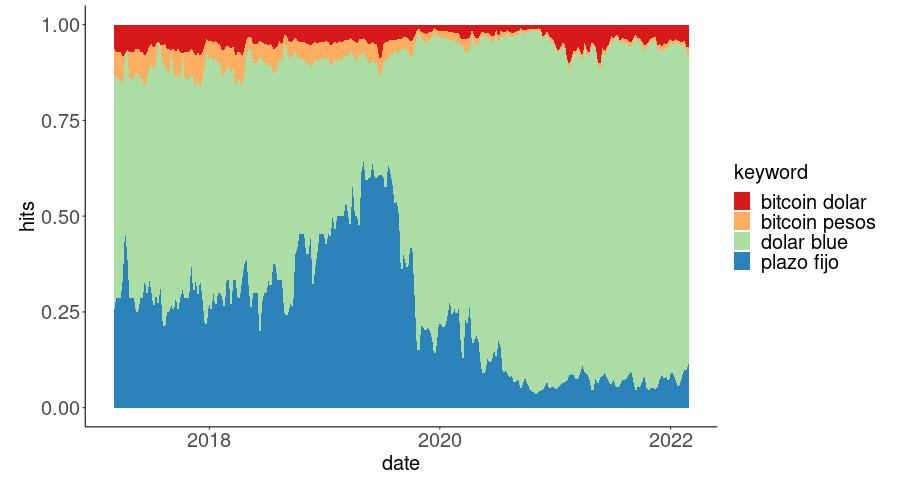
\includegraphics[width=1\textwidth]{images/C4/Rplot001.png}
     \end{center}
    \end{figure}
    
    \end{block}

    \end{column}
\end{columns}

\note{
\begin{itemize}
    \item Para poder dar respuestas a cada una de dichas preguntas se propone una evaluación conceptual y una evaluación empírica. 
    \item Evaluación conceptual
        \begin{itemize}
        \item Modelos OLG para los tres objetivos, con el mismo entorno (previsión perfecta, estacionariedad, un solo bien, dos generaciones que viven dos períodos, tiempo infinito).
        \end{itemize}
    \item Evaluación empírica
        \begin{itemize}
        \item Objetivo 1 y 2: técnicas de análisis de red
        \item Objetivo 3: datos de Google Trend (no hay posibilidad de georeferenciar datos de la blockchain o Twitter).
        \end{itemize}
\end{itemize}
}

\end{frame}
%----------